% How Medorama protects patient data: the principle, terms, Privacy Mode and the PHI permission,
% what is withheld and what replaces it (identifiers, pseudonyms, dates and ages, notes,
% searches, the administrator's choices), de-identifying files at the source (WFDB, MUSE, DICOM,
% EDF and BDF, files passed with a warning), the VitalStream viewer, exports and plug-ins,
% connected databases, failing closed, verification, limits, and the repository.
% Source: docs/protecting-patient-data.md; the code is the authority: medorama/src/server.rs
% (in_privacy, session_user, set_privacy, privacy, cleared, attachment_response,
% edf_deidentified), users.rs (in_privacy_mode), gate.rs, deid.rs, dicom.rs, pseudonyms.rs,
% gateway.rs (handle, shift_query, gate_annotations); tests: medorama/tests/privacy.rs,
% gateway.rs, connections.rs, dicom_samples.rs.
\chapter{How Medorama protects patient data}
\label{chap:protecting}

This chapter explains how Medorama keeps patients' identities from people who are not allowed to
see them. It is written for everyone who works with Medorama: users who want to know what
Privacy Mode shows, data managers who prepare data, and privacy officers and IT security
reviewers who must judge the design. The explanations are in plain language, and each section
ends with references to the code and the tests, for reviewers who want to check them. The
complete security review, with the threat model and the deployment checklist, is
\cref{chap:security}; the settings an administrator uses are described in
\cref{chap:users-privacy}.

\section{The principle}
\label{sec:protecting-principle}

Medorama brings together data that identify patients: names, medical record numbers, dates of
birth, account numbers, and the dates of every event. Its design rests on three rules.
\begin{enumerate}
\item \textbf{Identifiers are kept in one place only: the catalog database.} The catalog keeps
  every identifier as it was imported, in its own tables. Copies are not made elsewhere: the
  viewers, the waveform indexes, the results of analyses and the plug-in programs never receive
  them.
\item \textbf{What leaves the server is decided at the moment of sending.} Privacy Mode is a
  property of a user's session, not of the data. For each answer, the server checks who is
  asking and whether that session is in Privacy Mode, and then sends either the identified data
  or a de-identified copy made on the spot.
\item \textbf{Nothing identifying reaches the browser of a user who may not see it.} The page in
  the browser does no masking of its own: it never receives what it must not show. A user who
  opens the browser's developer tools, or calls the API directly, receives the same
  de-identified answers that the page displays.
\end{enumerate}
The part of the server that makes the de-identified copy is called the \textbf{privacy gate}
(\cref{fig:protecting-gate}).

\screenshot{privacy-gate.pdf}{The privacy gate: identifiers stay in the catalog's database, and
every answer of a session in Privacy Mode leaves through the gate, which replaces identifiers,
moves dates back, de-identifies files and refuses what it cannot clear.}{fig:protecting-gate}

\Cref{fig:protecting-compare} shows the same synthetic patient twice. On the left, an
administrator with the PHI permission sees the identified record. On the right, the same page in
Privacy Mode shows placeholders, a pseudonym and dates moved back by about a century.

\begin{figure}[htbp]
\centering
\begin{minipage}[t]{0.49\linewidth}\centering
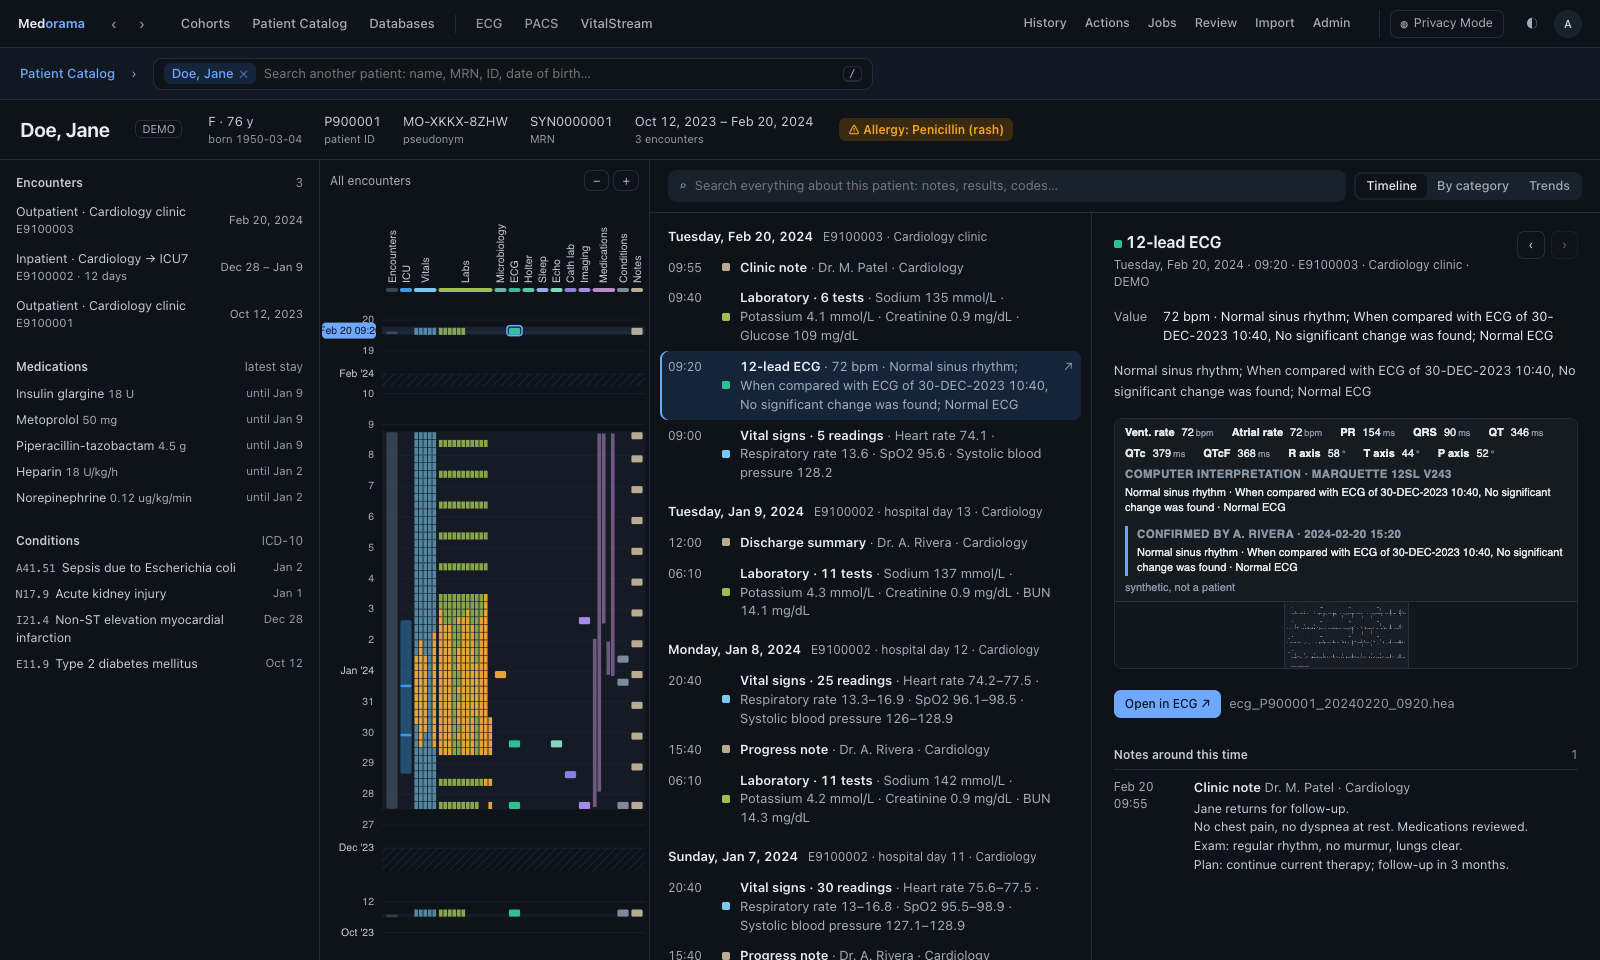
\includegraphics[width=\linewidth]{patient.png}
\end{minipage}\hfill
\begin{minipage}[t]{0.49\linewidth}\centering
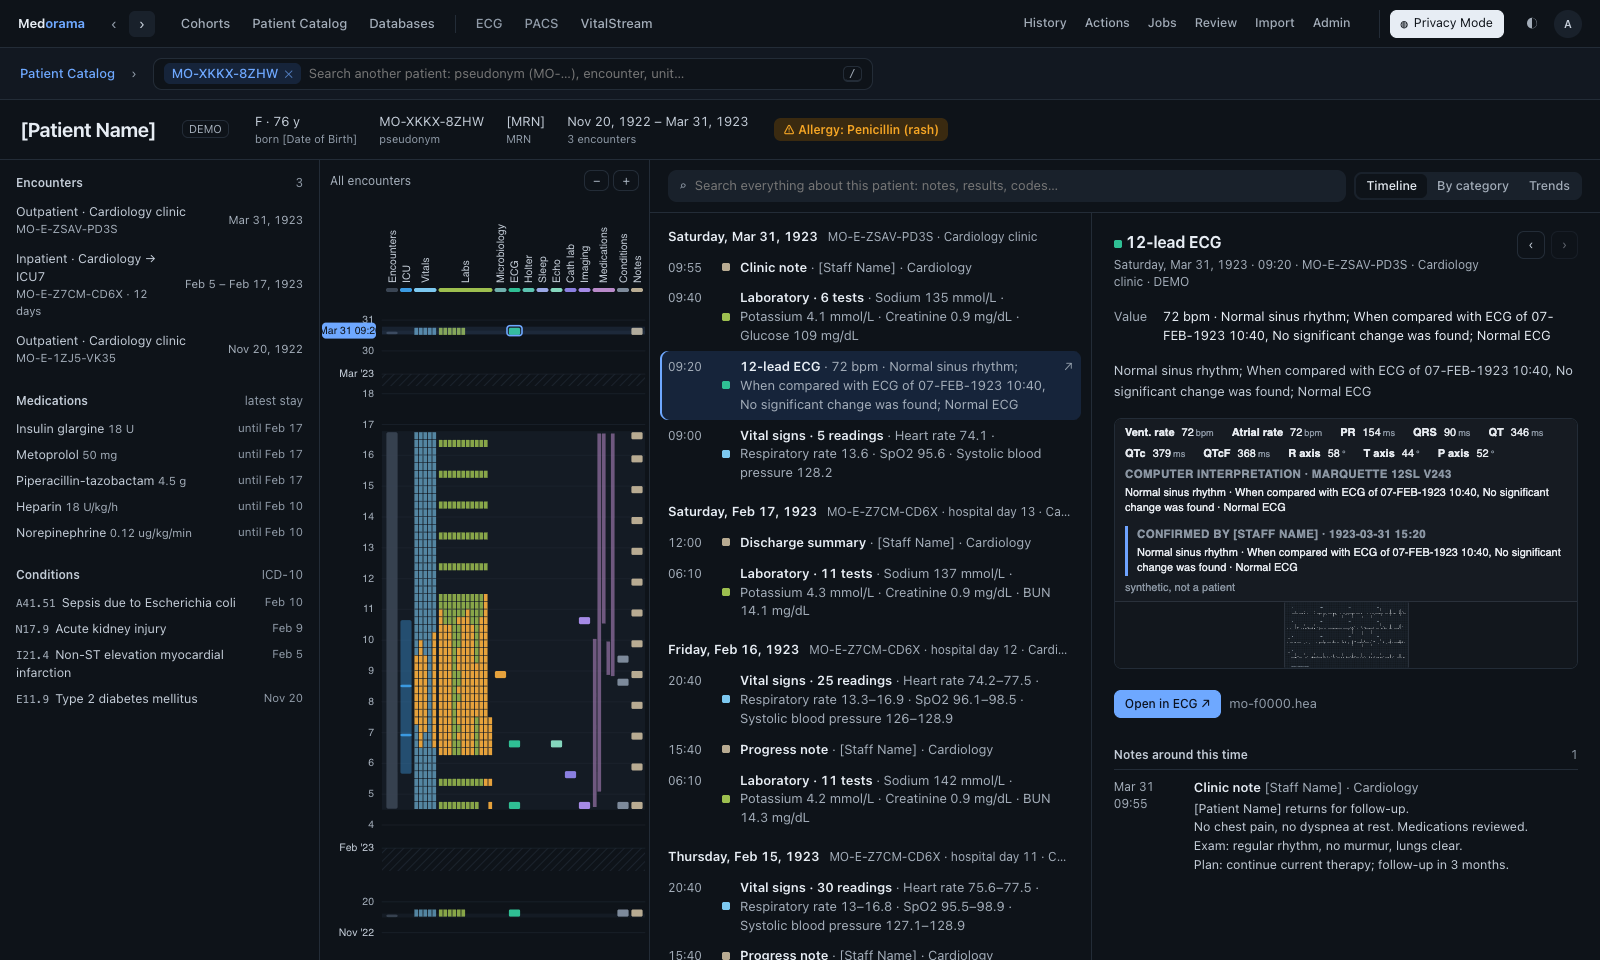
\includegraphics[width=\linewidth]{privacy.png}
\end{minipage}
\caption{The same synthetic patient, identified (left) and in Privacy Mode
(right).}\label{fig:protecting-compare}
\end{figure}

\section{Terms used in this chapter}
\label{sec:protecting-terms}

\begin{xltabular}{\linewidth}{@{}P{3.2cm}L@{}}
\caption{The terms of patient-data protection.}
\label{tab:protecting-terms}\\
\toprule
\tabhead Term & \tabhead Meaning \\
\midrule
\endfirsthead
\toprule
\tabhead Term & \tabhead Meaning \\
\midrule
\endhead
\bottomrule
\endfoot
PHI & Protected health information: anything that can identify a patient, together with their
  health data. \\
Catalog & Medorama's own database of patients, encounters, clinical entries, recordings, users
  and the audit log (SQLite or PostgreSQL). \\
Identifier & A value that names a person directly: a name, a medical record number (MRN), a date
  of birth, an account number (CSN), an imported patient or encounter ID. \\
PHI permission & A right that an administrator gives to a user account. Without it, a user can
  never see identifiers. \\
Privacy Mode & The state of a session in which every answer passes the privacy gate. \\
Privacy gate & The server code that de-identifies answers and files for sessions in Privacy
  Mode, and refuses what it cannot de-identify. \\
Pseudonym & A random code that stands for a patient (\code{MO-XXXX-XXXX}) or an encounter
  (\code{MO-E-XXXX-XXXX}) in Privacy Mode. \\
Placeholder & Fixed text that stands for a withheld value, such as \code{[Patient Name]} or
  \code{[MRN]}. \\
Date offset & The amount by which Privacy Mode moves a patient's dates back: the catalog's
  offset plus the patient's own number of days. \\
Connected database & A database that Medorama reads in place, such as an OMOP instance, instead
  of importing it. \\
\end{xltabular}

\section{Privacy Mode and the PHI permission}
\label{sec:protecting-modes}

Every session is in Privacy Mode unless its user has the PHI permission and has switched Privacy
Mode off. \Cref{tab:protecting-who} gives the defaults.

\begin{xltabular}{\linewidth}{@{}P{6.6cm}L@{}}
\caption{Who is in Privacy Mode.}
\label{tab:protecting-who}\\
\toprule
\tabhead User & \tabhead Privacy Mode \\
\midrule
\endfirsthead
\toprule
\tabhead User & \tabhead Privacy Mode \\
\midrule
\endhead
\bottomrule
\endfoot
Without the PHI permission (any role) & Always on. It cannot be switched off. \\
With the PHI permission, not an administrator & On when the user signs in. The user may switch
  it off. \\
Administrator with the PHI permission & Off when the user signs in. The administrator may switch
  it on. \\
\end{xltabular}

The role of a user (viewer, analyst or administrator) decides what the user may \emph{do}; the
PHI permission decides what the user may \emph{see}. An administrator grants the PHI permission
when creating an account, or later in \ui{Admin} $\rightarrow$ \ui{Users}
(\cref{chap:users-privacy}). Most users should not have it: they work with pseudonyms and shifted
dates, which is enough for most research.

\paragraph{Switching Privacy Mode.} The \ui{Privacy Mode} switch in the page's header changes the
mode for that session. The server keeps the choice with the session, never in the browser, and
writes an entry to the audit log (\code{privacy\_on} or \code{privacy\_off}): leaving Privacy
Mode is always audited. The page then reloads, so that nothing identified stays on the screen
after Privacy Mode is switched on. A user without the PHI permission who asks to leave Privacy
Mode is refused (HTTP 403). Every sign-in starts in the user's default mode, so whoever uses the
browser next starts there too. Signing out, or a session that ends while the page is open,
reloads the page: the next person to sign in at that browser sees nothing of what the previous
user saw.

A session in Privacy Mode is treated exactly like a user without the PHI permission: the server
replaces the session's user with a copy that has no PHI permission (\file{users.rs},
\code{User::in\_privacy\_mode}), so every check that depends on the permission fails closed for
that session.

\paragraph{For reviewers.} The decision is \file{server.rs} \code{in\_privacy} and
\code{session\_user}; the switch is \file{server.rs} \code{set\_privacy}. It is tested in
\file{medorama/tests/privacy.rs}: a user without the permission is refused, and an administrator
who switches Privacy Mode on receives no identifier.

\section{What is withheld and what replaces it}
\label{sec:protecting-withheld}

\subsection{Identifiers and dates}
\label{sec:protecting-identifiers}

\Cref{tab:protecting-replaced} lists what Privacy Mode withholds by default and what the user sees
instead. The defaults follow the identifiers of the HIPAA Safe Harbor list that the catalog
holds, with one exception, the text of notes, described in \cref{sec:protecting-notes}.

\begin{xltabular}{\linewidth}{@{}P{5.0cm}L@{}}
\caption{What Privacy Mode withholds, and what replaces it.}
\label{tab:protecting-replaced}\\
\toprule
\tabhead Data & \tabhead In Privacy Mode \\
\midrule
\endfirsthead
\toprule
\tabhead Data & \tabhead In Privacy Mode \\
\midrule
\endhead
\bottomrule
\endfoot
Patients' names & \code{[Patient Name]} \\
Staff names (authors of notes, ECG overreaders, physicians) & \code{[Staff Name]} \\
Medical record numbers & \code{[MRN]} \\
Account numbers (CSN) & \code{[CSN]} \\
Dates of birth & \code{[Date of Birth]}. The age is computed on the server and shown instead. \\
Imported patient IDs & The patient's pseudonym, \code{MO-XXXX-XXXX}, because an imported ID may
  be an MRN. In a database's own columns, \code{[Patient ID]}. \\
Imported encounter IDs & The encounter's pseudonym, \code{MO-E-XXXX-XXXX}. \\
Every date and time & Moved back by the patient's date offset (\cref{sec:protecting-dates}). \\
Ages above 89 & \code{90+} \\
Recordings' paths and file names & Tokens (\code{mo-rec:<n>}, \code{mo-f0003.dcm}), and
  \code{[Recording]} or \code{[File Name]} where a name is shown. \\
An identifier found inside text & The same replacement wherever it appears (MRNs, account
  numbers, and imported IDs of four or more characters that contain a digit). \\
Columns of imported databases that hold identifiers & Kept under their imported names. Their
  cells become placeholders, so the table keeps the shape of the source. \\
Columns that the catalog does not recognize & Withheld (\code{[Withheld]}), except measurement
  columns such as \code{QT (ms)}, which hold numbers. In the \ui{Databases} tab, the search, the
  filters and the sorting skip such columns. \\
The text of notes and reports & Shown by default, with the patient's own names and date of birth
  replaced, and marked with a warning. Withheld (\code{[Withheld]}) when the administrator
  chooses so (\cref{sec:protecting-notes}). \\
\end{xltabular}

Placeholders are fixed text. They never reveal the length or the form of the value they replace.

\subsection{Pseudonyms}
\label{sec:protecting-pseudonyms}

Each patient receives a pseudonym such as \code{MO-D5QM-Y1X5} when first seen, and each encounter
one such as \code{MO-E-QMC6-E2VA}. In Privacy Mode, users find patients by these pseudonyms, and
exports name patients by them.
\begin{itemize}
\item \textbf{Random and stored, never derived.} The seven characters come from the operating
  system's secure random generator, and an eighth is a check character. No calculation on an MRN
  or a name produces the pseudonym: the only link between a pseudonym and a person is the catalog
  database. This follows HIPAA 45 CFR \S164.514(c), which asks that a re-identification code not
  be ``derived from or related to information about the individual'', and ISO/TS 25237.
\item \textbf{Why not a hash of the MRN.} MRNs are short, so every possible MRN can be hashed in
  minutes, which would reverse an unkeyed hash. A keyed hash would depend on one secret forever
  and would still be derived from the identifier.
\item \textbf{Stable.} A patient keeps the same pseudonym through re-imports and restarts. When
  two records are merged as one person, the absorbed record's pseudonym stays as an alias, so
  that earlier exports and cohort definitions still resolve.
\item \textbf{Checked.} The check character (Luhn mod 32, in Crockford's base 32, which has no I,
  L, O or U) catches any single mistyped character, so a pseudonym typed into a search is either
  right or refused.
\item \textbf{The same everywhere.} Pages, exports, cohort definitions and their history, DICOM
  headers and plug-ins' job descriptions use the same pseudonym.
\end{itemize}
A catalog rebuilt from scratch draws new pseudonyms and new date offsets. Keep backups of the
database to keep them stable (\cref{sec:deployment-backups}).

\subsection{Dates and ages}
\label{sec:protecting-dates}

Research depends on the time between events, so Privacy Mode moves dates rather than removing
them.
\begin{itemize}
\item \textbf{The catalog's offset.} Every date and time moves back by an offset that the
  administrator sets in years, months, days and hours (\ui{Admin} $\rightarrow$ \ui{Privacy
  Mode}). It is counted on the calendar from 2000-01-01. The default is 36\,570 days, about 100
  years.
\item \textbf{Each patient's own days.} On top of that, each patient's dates move back by a whole
  number of days between 0 and a maximum (\code{spread\_days}: 365 by default, at least 30 and
  at most 3650; a smaller value saved before that minimum is kept, since raising it moves every
  patient's dates, and \cmd{medorama serve} warns about it at start). This number is drawn at
  random once, when the patient's
  pseudonym is drawn, and stored with it. Every user and every session therefore sees the same
  dates for the same patient. Something that names no patient moves by the catalog's offset
  alone.
\item \textbf{Intervals are kept.} The time between any two events of one patient is exact.
  Between two patients, it changes by the difference of their own days.
\item \textbf{Row by row.} A patient's pages and files move by that patient's offset; a list or an
  export moves row by row, by the patient each row names; a recording in VitalStream moves by the
  patient of its encounter.
\item \textbf{Everywhere.} Dates move in every form the catalog holds or sends: numbers (Unix
  times), text (\code{2024-01-02} with or without a time, \code{2024/01/02}, \code{01/02/2024},
  \code{2.1.2024}, \code{02-JAN-2024}, \code{Jan 2, 2024}, \code{2 January 2024},
  \code{20240102}), BedMaster file names' Unix times (a name whose moved time falls before 1970
  is written with a minus sign: \code{ICU7\_12--1455465600}), DICOM dates and times, GE MUSE XML
  dates, WFDB base dates, EDF start dates, and the keys of entries that carry a time
  (\code{labs:<encounter>:<time>}). A date written \code{01/02/2024} is read month first, unless
  the catalog writes dates day first (\ui{Admin} $\rightarrow$ \ui{Dates and times}) or the
  month would be over 12; \code{2.1.2024} is read day first. Either way the year moves back by
  about a century, so a misread date shows no real date. A Unix time written on its own is a
  number, and is kept.
\item \textbf{Searches and criteria in Privacy Mode.} A search, a filter or a sort uses only what
  the session is shown (pseudonyms, file tokens, each patient's dates as shown), so it cannot test
  a real value. A date a user types, in a cohort criterion or a date filter, is a date as shown:
  the server compares it with each patient's dates as that session sees them, so the criterion
  means exactly what the page says. The page never holds the date offset: only administrators
  may read it (\code{GET deid}).
\item \textbf{Ages} are computed on the server from the date of birth, which never leaves it.
  Ages above 89 are shown as \code{90+}.
\end{itemize}

\begin{note}
Date shifting is pseudonymization, not anonymization. Anyone who learns the real date of one of a
patient's events can re-date all of that patient's events, and every other patient's to within
\code{spread\_days}. Record the offset under your governance, and keep it confidential.
\end{note}

\subsection{Text and notes}
\label{sec:protecting-notes}

Free text, such as clinical notes and reports, can name the patient, relatives or staff in ways
that no rule can recognize reliably. By default, Privacy Mode shows the text of notes, because it
is often essential for research, with the following protections:
\begin{itemize}
\item the patient's own names (each word of at least two letters, and each part of a compound
  name such as \code{Smith-Jones} or \code{O'Brien}) and date of birth are replaced by
  \code{[Patient Name]} and \code{[Date of Birth]};
\item identifiers the catalog knows (MRNs, account numbers, imported IDs of four or more
  characters that contain a digit) are replaced wherever they appear, and so are recordings'
  paths and the folders they lie in (\code{[Folder]}), which may be named after the patient;
\item phrases such as ``Confirmed by \dots'' or ``Signed by \dots'' are replaced by
  \code{[Staff Name]};
\item dates in the text are moved back;
\item the page marks the text with a warning, because it may still identify someone.
\end{itemize}
An administrator who prefers to withhold all free text ticks \ui{The text of notes and reports}
in \ui{Admin} $\rightarrow$ \ui{Privacy Mode}. Notes then appear as \code{[Withheld]}, and their
text is not searched in Privacy Mode. The same choice applies to the annotations of EDF+
recordings shown in VitalStream (\cref{sec:protecting-vitalstream}).

\subsection{Searches}
\label{sec:protecting-searches}

In Privacy Mode, a search by name, MRN, date of birth, account number or a withheld column is
refused with a message (HTTP 400). A plain word does not match identifiers behind the scenes
either: otherwise the number of results would reveal whether a person is in the catalog.
Patients are found by their pseudonyms, and encounters by theirs. Every search, filter and sort
uses only what the session is shown: pseudonyms, tokens and placeholders, and each patient's
dates as they are shown, so a search for a real identifier or a real date finds nothing, and
lists are ordered by the dates shown. Searches of identifiers by users who may see them are
written to the audit log (\code{phi\_search}), and so are searches, filters and cohort criteria
made in Privacy Mode, with their text (\code{privacy\_search}).

\subsection{What the administrator can change}
\label{sec:protecting-settings}

\ui{Admin} $\rightarrow$ \ui{Privacy Mode} lets an administrator choose which kinds of identifiers
are withheld, the catalog's offset and \code{spread\_days} (\cref{sec:users-privacy-settings}).
Every change is written to the audit log (\code{deid\_settings}) with the new settings. Some
protections do not depend on these settings and always apply in Privacy Mode: imported patient
and encounter IDs become pseudonyms, file names become tokens, staff names become
\code{[Staff Name]}, unrecognized columns are withheld, and files that the gate cannot
de-identify are refused.

\paragraph{For reviewers.} Placeholders, the identifier dictionary and table cells are in
\file{gate.rs} (\code{Dict}, \code{Restricted::json}, \code{column\_placeholder},
\code{column\_mask}); dates, ages and the settings in \file{deid.rs} (\code{FIELDS},
\code{Settings}, \code{answer\_with}, \code{shift\_text}); pseudonyms in \file{pseudonyms.rs}.
Each module has unit tests, and \file{medorama/tests/privacy.rs} tests them end to end.

\section{De-identifying files at the source}
\label{sec:protecting-files}

Patients' files (ECGs, recordings, DICOM studies, documents) are sent one item at a time, through
\code{patients/\{id\}/file/\{item\}}, and only the files that belong to that item. In Privacy
Mode, the gate decides how each file leaves according to its kind
(\cref{tab:protecting-files}). A file is de-identified as it is sent; the original on disk is
never changed.

\begin{xltabular}{\linewidth}{@{}P{3.6cm}L@{}}
\caption{How each kind of file leaves in Privacy Mode.}
\label{tab:protecting-files}\\
\toprule
\tabhead Kind of file & \tabhead In Privacy Mode \\
\midrule
\endfirsthead
\toprule
\tabhead Kind of file & \tabhead In Privacy Mode \\
\midrule
\endhead
\bottomrule
\endfoot
WFDB header (\file{.hea}) & Comments that identify the patient (name, ID, MRN, date of birth,
  address, phone, however their key is written: \code{Patient\_Name:}, \code{Name=},
  \code{Patient name -}, \code{Birthdate:}) are removed; the patient's own names and date of
  birth are replaced in every other comment; staff named in comments become
  \code{[Staff Name]}; the base date and dates in comments are moved back; ages above 89 become
  \code{90+}; the record's name and its signal files' names are replaced by tokens. \\
WFDB samples (\file{.dat}) & Sent as they are (they hold only numbers) when a header of the same
  item names them; any other \file{.dat} file is refused. \\
GE MUSE XML (\file{.xml} with a \code{RestingECG} element) & The patient's demographics are
  removed except age (capped) and sex, whatever attributes or spaces their tags hold; the order
  is removed; staff names become \code{[Staff Name]} and their IDs are emptied; a patient's name
  elsewhere becomes \code{[Patient Name]}; the patient's own names and date of birth are replaced
  in the statements; ``Confirmed by'' phrases are replaced; every date is moved back. A file that
  still holds a patient's name, ID or date of birth after all this is refused, as is any other
  XML file. \\
DICOM (\file{.dcm}, \file{.dicom}, or a file recognized by its content) & The header is
  rewritten with the actions of the DICOM confidentiality profile for the attributes listed
  (\cref{sec:protecting-dicom}); the pixel data are copied byte for byte. The file is marked as
  possibly identifying. \\
EDF, EDF+, BDF, BDF+ (\file{.edf}, \file{.bdf}) & The header is de-identified and the texts of
  annotations are removed; the samples are sent as they are (\cref{sec:protecting-edf}). \\
Pictures, videos and PDF documents & Sent as they are, marked as possibly identifying: the
  viewer's tab shows an amber warning triangle. \\
Anything else & Refused (HTTP 403). \\
\end{xltabular}

\paragraph{File names never leave.} In Privacy Mode, an item's files are named by tokens
(\code{mo-f0000.hea}, \code{mo-f0001.dat}), and a request that gives a real file name is not
accepted. Answers that carry files vary with the session cookie (\code{Vary: Cookie}), so a
browser never shows a cached identified copy in Privacy Mode.

\subsection{DICOM}
\label{sec:protecting-dicom}

The rewrite applies the actions of DICOM PS3.15 Table E.1-1, the \textbf{Basic Application
Level Confidentiality Profile} (\code{X}: removed; \code{Z}: emptied; \code{D}: a dummy value;
\code{U}: a new UID), for the attributes listed in \file{dicom.rs} (\code{PROFILE}), with the
\textbf{Retain Longitudinal Temporal Information with Modified Dates} option: dates are moved by
the patient's date offset, instead of removed (\cref{tab:protecting-dicom}). It is not a
certified implementation of the profile: an attribute of the table that the list lacks is kept,
with its free text scrubbed as below. The De-identification Method written into the file says
so.

\begin{xltabular}{\linewidth}{@{}P{5.6cm}L@{}}
\caption{DICOM elements in Privacy Mode.}
\label{tab:protecting-dicom}\\
\toprule
\tabhead Element & \tabhead In Privacy Mode \\
\midrule
\endfirsthead
\toprule
\tabhead Element & \tabhead In Privacy Mode \\
\midrule
\endhead
\bottomrule
\endfoot
Patient's Name & \code{[Patient Name]} \\
Patient ID & The patient's pseudonym \\
Patient's Birth Date & Emptied \\
Patient's Age & Capped at 90 years when ages are capped \\
Patient's Sex, Size and Weight & Kept \\
Every other element of the patient group (0010) & Removed \\
The clinical trial module (0012) & Removed \\
Other person names (referring, performing and reading physicians, operators, observers) &
  \code{[Staff Name]} \\
The attributes of the list: institution, department, station, addresses and phones, device,
  detector and other equipment IDs, accession, study, order, procedure, admission and visit IDs;
  descriptions (study, series, requested and performed procedures, derivation, admitting and
  discharge diagnoses); comments (image, study, acquisition, identifying, performed procedure
  step, visit); protocol names; structured report text and content (Text Value, Content
  Sequence); graphic annotations; icon images; digital signatures & Removed (\code{X}), or
  emptied (\code{Z}: accession, institution name, study ID, order numbers) \\
Curves (50xx), overlays (60xx: their bitmaps, labels and comments), the retired results group
  (4008) & Removed \\
Free text left (SH, LO, ST, LT, UC, UT; in implicit-VR files, elements of unknown VR that hold
  text) & The patient's own names and date of birth, and the identifiers the catalog knows,
  replaced; dates in it moved back \\
Private elements & Removed \\
Instance UIDs (study, series, instance, frame of reference, references) & Replaced by
  \code{2.25.} and 128 bits of an HMAC-SHA-256 under the catalog's secret, so that a series still
  holds together and nobody without the secret can map them back. The standard's own UIDs
  (classes, transfer syntaxes) are kept. \\
Dates and times & Moved back, a date and its time together \\
Patient Identity Removed, De-identification Method, Longitudinal Temporal Information Modified &
  Added (\code{YES}, the method, \code{MODIFIED}) \\
\end{xltabular}

The file keeps its transfer syntax (explicit or implicit VR little endian, and every compressed
syntax). In implicit VR the file does not say which elements are person names: the rewrite knows
the person names of the standard's dictionary by their tags. Deflated and big-endian files are
refused, because they could not be rewritten safely, and so are files with sequences nested more
than 32 deep.
Real files from several vendors and syntaxes (CT in implicit and explicit VR, JPEG Lossless, JPEG
Extended 12-bit, multi-frame JPEG Baseline angiography, panoramic X-ray) were checked with pydicom
after the rewrite: no original identifier and no private element remained, and the pixels were
identical (\file{medorama/tests/dicom\_samples.rs}).

What the pixels show is not changed. Ultrasound images, secondary captures and scanned documents
may carry names burned into the image, so every DICOM file is sent with the ``may contain PHI''
mark.

\subsection{EDF and BDF}
\label{sec:protecting-edf}

An EDF or BDF header has two identification fields of 80 characters, one for the patient and one
for the recording, and states the recording's start date and time
(\cref{sec:recordings-edf}). In Privacy Mode, a file sent to the browser is rewritten as follows
(\file{deid.rs} \code{edf\_header} and \code{edf\_annotations}, called by \file{server.rs}
\code{edf\_deidentified}):
\begin{itemize}
\item the patient field becomes \code{X X X X}, EDF+'s form for an anonymous patient;
\item in EDF+ and BDF+ files, the recording field becomes \code{Startdate dd-MMM-yyyy X X X},
  with the start date moved back; in plain EDF and BDF files, whose recording field is free
  text, it is left blank;
\item the start date and time are moved back. EDF writes two-digit years for 1985 to 2084 only:
  an EDF+ file whose moved date falls outside that range has \code{yy} in its date field and the
  full year in its recording field, as EDF+ prescribes, and a plain EDF file states no start date
  rather than a wrong one;
\item in EDF+ and BDF+ files, the texts of annotations are removed. Each data record keeps only
  its time-keeping annotation (its onset), so that the file's timing stays whole; the bytes after
  the last whole data record are left out;
\item the samples are sent as they are.
\end{itemize}
A file without annotation signals is streamed, and only its header is rewritten. A file with
annotation signals is rewritten whole in memory, so EDF+ files with annotations larger than 64\,MB
are refused in Privacy Mode; such recordings can still be opened in VitalStream. The technical
fields of the signal headers (labels, units, transducer and prefiltering descriptions) are kept
as they are.

The engine and the viewers never put the patient and recording fields into an index or into any
answer. Medorama's \code{identify} action reads them into the catalog's identifier tables, where
an administrator can check that the file belongs to the patient it is linked to
(\cref{chap:administration}).

\subsection{Why some files pass with a warning}
\label{sec:protecting-warning}

Pictures, videos, PDF documents and DICOM pixels are images: the gate cannot read what they show,
and removing burned-in text would require optical character recognition, which Medorama does not
do. Refusing them would make imaging research impossible in Privacy Mode, so they are sent as they
are, with the header \code{x-medorama-may-contain-phi}, and the page shows an amber warning
triangle on the tab that displays them. Every other kind of file that the gate cannot de-identify
is refused.

\paragraph{For reviewers.} The file rules are \file{gate.rs} \code{FileKind} and
\code{file\_kind}, and \file{server.rs} \code{attachment\_response}. WFDB headers are
\file{deid.rs} \code{wfdb\_header}; MUSE XML is \file{deid.rs} \code{muse\_xml}; DICOM is
\file{dicom.rs}; EDF is \file{deid.rs} \code{edf\_header} and \code{edf\_annotations}, called by
\file{server.rs} \code{edf\_deidentified}. File tokens are \file{gate.rs} \code{file\_token} and
\code{token\_index}.

\section{The VitalStream viewer}
\label{sec:protecting-vitalstream}

The VitalStream waveform viewer runs as a separate program on the server, reachable only through
Medorama's \emph{gateway} (\file{/viewer/}; \cref{sec:architecture-gateway}). The viewer itself
never reads names or dates of birth from any recording. In Privacy Mode, the gateway adds the
following rules:
\begin{itemize}
\item recordings are opened by token (\code{mo-rec:<n>}), never by path, and a path sent by the
  page is refused;
\item browsing and scanning folders is refused, because folder and file names may identify;
\item the times that the page sends are moved forward before they reach the viewer, and every
  time in the viewer's answers is moved back, by the recording's patient's date offset;
\item a dataset's path and name are replaced by its token and \code{[Recording]};
\item the annotations of EDF+ and BDF+ recordings, which are free text and are shown as events in
  VitalStream's Annotations lane, are treated like notes: when Privacy Mode withholds the text of
  notes, each annotation reads \code{[Annotation]}; otherwise the patient's own names and date of
  birth are replaced (\file{gateway.rs}, \code{gate\_annotations});
\item every answer then passes the gate's last layer, like any other answer, which replaces the
  identifiers the catalog knows and moves dates back.
\end{itemize}

\paragraph{For reviewers.} \file{gateway.rs} (\code{handle}, \code{shift\_query},
\code{gate\_annotations}, with its unit test \code{annotations\_in\_privacy\_mode}); tested with a
real viewer in \file{medorama/tests/gateway.rs}.

\section{Exports and plug-in actions}
\label{sec:protecting-exports}

\begin{itemize}
\item \textbf{Exports} made in Privacy Mode (cohort members, definitions, members' data, Excel
  files, database CSV files) pass the same gate. They have the same columns as identified
  exports, with identifiers as placeholders, patients named by pseudonym and dates moved back,
  and their file names end in \code{-privacy}. Exports by users who see identifiers are written
  to the audit log (\code{phi\_export}).
\item \textbf{Plug-in actions}, programs that an administrator installs to analyze recordings,
  receive a job description with the recording's path, its index folder, an output folder, and
  the pseudonyms of its encounters and patients, never their imported IDs (\cref{chap:actions}).
  They also do not receive the server's secrets in their environment
  (\cref{sec:security-jobs}).
\end{itemize}

\section{Connected databases}
\label{sec:protecting-connected}

A connected database (an OMOP instance, a data warehouse read through SQL views) is read in
place, read-only, and its data leave through the same gate as the catalog's.
\begin{itemize}
\item \textbf{Only canonical columns are read.} Medorama reads a connected database through three
  views of fixed columns (persons, visits, entries), each column with a privacy class: key,
  identifier, date, free text, staff or clinical value. A view cannot add a field that the gate
  does not know (\cref{chap:connecting}).
\item \textbf{Persons are linked to patients.} A connected database's persons are linked to the
  catalog's patients, so they leave as pseudonyms. Their identifiers are copied into the
  catalog's identifier tables, where the gate knows them, and their keys in the source database
  never leave.
\item \textbf{Entries are named by tokens.} An entry is named by a keyed hash
  (\code{live:<connection>:<token>}) that holds neither its key nor its time. Its dates move back
  with the rest, its text follows the rule for notes, and its authors are treated as staff.
\item \textbf{Searches} of identifiers in connected databases need the PHI permission, as in the
  catalog.
\end{itemize}

\paragraph{For reviewers.} \file{sources/} (read-only sessions, views, the person registry in
\file{sources/link.rs}) and \file{patient/items.rs} \code{live\_items}; tested in
\file{medorama/tests/connections.rs} over a synthetic OMOP database, in SQLite and PostgreSQL.

\section{Failing closed}
\label{sec:protecting-fail-closed}

Most answers are de-identified by the code that builds them, because that code knows what each
value is. A last layer of the server then enforces the rule for every answer of a session in
Privacy Mode:
\begin{itemize}
\item a JSON answer passes through the gate there, whatever the endpoint;
\item a file passes only if the gate cleared it;
\item any other answer that carries data is refused (HTTP 403), and the refusal is written to the
  server's error output.
\end{itemize}
The pages and scripts of the web interface, redirects and error messages hold no patient data and
pass unchanged. As a result, a new endpoint whose author forgets the gate cannot leak identifiers:
its answer is either refused or de-identified. This is why the gate is said to \emph{fail
closed}. In the same spirit, a session in Privacy Mode is handled as a user without the PHI
permission, so a forgotten permission check also errs on the side of withholding.

\paragraph{For reviewers.} \file{server.rs} \code{privacy} (the last layer), and \code{cleared}
and \code{may\_hold\_phi} (the marks set by handlers). The internal header
\code{x-medorama-gate} is removed before an answer leaves.

\section{How the design is verified}
\label{sec:protecting-verified}

\begin{itemize}
\item \textbf{End to end.} \file{medorama/tests/privacy.rs} seeds a catalog with identifiers that
  cannot appear by chance: a name, an MRN, patient, encounter and account numbers, a date of
  birth, staff names, an institution, and real dates in the forms that tables, DICOM, MUSE, WFDB,
  EDF and EDF+ write them. They are placed in every format the catalog serves: tables, notes, a
  WFDB record, GE MUSE XML, DICOM, an EDF+ file, a picture, a text file and an ICU recording. The
  test then requests every page's answers, every entry's detail, every file and its parts, and
  every cohort and database export, as a user without the PHI permission and as an administrator
  who switched Privacy Mode on. It asserts that no byte of any answer holds any of the seeded
  identifiers, that no JSON number is a real time, that identifier searches are refused or find
  nobody, that placeholders and pseudonyms appear, that the text file is refused, and that
  pictures and DICOM files are marked. It also checks that the identified answers do hold the
  identifiers, so that the test would fail if it checked nothing.
\item \textbf{The viewer.} \file{medorama/tests/gateway.rs} runs a real VitalStream viewer behind
  the gateway, in Privacy Mode too.
\item \textbf{Connected databases.} \file{medorama/tests/connections.rs} repeats the Privacy Mode
  check over a synthetic OMOP database.
\item \textbf{Each de-identifier.} Unit tests in \file{gate.rs}, \file{deid.rs} (including real
  EDF test files), \file{dicom.rs}, \file{pseudonyms.rs} and \file{gateway.rs};
  \file{medorama/tests/dicom\_samples.rs} checks real DICOM files with pydicom.
\end{itemize}
The commands that run these tests are listed in \cref{sec:security-verifying}.

\section{What Privacy Mode cannot do}
\label{sec:protecting-limits}

Privacy Mode reduces what users see; it does not make data anonymous. Reviewers and users should
know its limits.
\begin{itemize}
\item \textbf{Burned-in text.} Names written into pictures, scanned PDFs, video frames and DICOM
  pixels are not removed. These files are marked with the amber warning instead.
\item \textbf{Free text.} Notes, reports and EDF+ annotations may name the patient, relatives or
  staff in ways that no rule recognizes. They are marked where they are shown, and an
  administrator can withhold them entirely.
\item \textbf{Quasi-identifiers.} Sex, a capped age, rare diagnoses, units and beds, small cohorts
  and exact intervals can single out a person when combined with outside knowledge.
\item \textbf{Date offsets.} Learning one real date of a patient reveals that patient's offset,
  and every other patient's to within \code{spread\_days}.
\item \textbf{Not Safe Harbor.} Because dates are shifted rather than removed, data viewed or
  exported in Privacy Mode are not de-identified under HIPAA's Safe Harbor method. They suit use
  as a limited data set under a data use agreement, or under an expert determination
  (\cref{sec:security-regulatory}).
\item \textbf{Everyone sees every patient.} Medorama has no per-patient or per-study access
  lists: every signed-in user may see every patient of a catalog, as Privacy Mode and the PHI
  permission allow. Separate catalogs serve separate studies.
\end{itemize}

\begin{phibox}
The deploying institution remains responsible for the rest: who receives accounts and the PHI
permission, how the server and its backups are protected, which data are imported, and how
exports are used and shared. The deployment checklist (\cref{sec:security-checklist}) lists these
duties. Treat what a session in Privacy Mode exports as pseudonymized data, not as anonymous
data.
\end{phibox}

\section{The repository holds no patient data}
\label{sec:protecting-repository}

Medorama's source repository contains no patient data. Tests and demonstrations use synthetic
data only, or public data sets kept outside the repository. A privacy check
(\file{tools/git-hooks/check-files}), run by the pre-commit and pre-merge-commit hooks on what
git would store, refuses recordings, data files, DICOM and MUSE XML files (recognized by their
content), notebooks with outputs, real recording names and anything in a \file{sample\_data/}
folder. CI runs the same check on every commit of each pull request and push, and on every file
(\file{.github/workflows/checks.yml}), so a commit made without the hooks is still caught before
it is merged. The rules are in the repository's \file{PRIVACY.md}.
